%%%%%%%%%%%%%%%%%%%%%%%%%%%%%%%%%%%%%%%%%
% Journal Article
% LaTeX Template
% Version 1.4 (15/5/16)
%
% This template has been downloaded from:
% http://www.LaTeXTemplates.com
%
% Original author:
% Frits Wenneker (http://www.howtotex.com) with extensive modifications by
% Vel (vel@LaTeXTemplates.com)
%
% License:
% CC BY-NC-SA 3.0 (http://creativecommons.org/licenses/by-nc-sa/3.0/)
%
%%%%%%%%%%%%%%%%%%%%%%%%%%%%%%%%%%%%%%%%%

%----------------------------------------------------------------------------------------
%	PACKAGES AND OTHER DOCUMENT CONFIGURATIONS
%----------------------------------------------------------------------------------------

\documentclass[]{article}
\usepackage{blindtext} % Package to generate dummy text throughout this template

\usepackage[sc]{mathpazo} % Use the Palatino font
\usepackage[T1]{fontenc} % Use 8-bit encoding that has 256 glyphs
\linespread{1.05} % Line spacing - Palatino needs more space between lines
\usepackage{microtype} % Slightly tweak font spacing for aesthetics

\usepackage[english]{babel} % Language hyphenation and typographical rules

\usepackage[hmarginratio=1:1,top=32mm,columnsep=20pt]{geometry} % Document margins
\usepackage[hang, small,labelfont=bf,up,textfont=it,up]{caption} % Custom captions under/above floats in tables or figures
\usepackage{booktabs} % Horizontal rules in tables

\usepackage{lettrine} % The lettrine is the first enlarged letter at the beginning of the text

\usepackage{enumitem} % Customized lists
\setlist[itemize]{noitemsep} % Make itemize lists more compact

\usepackage{abstract} % Allows abstract customization
\renewcommand{\abstractnamefont}{\normalfont\bfseries} % Set the "Abstract" text to bold
\renewcommand{\abstracttextfont}{\normalfont\small\itshape} % Set the abstract itself to small italic text

\usepackage{titlesec} % Allows customization of titles
\renewcommand\thesection{\Roman{section}} % Roman numerals for the sections
\renewcommand\thesubsection{\roman{subsection}} % roman numerals for subsections
\titleformat{\section}[block]{\large\scshape\centering}{\thesection.}{1em}{} % Change the look of the section titles
\titleformat{\subsection}[block]{\large}{\thesubsection.}{1em}{} % Change the look of the section titles

\usepackage{fancyhdr} % Headers and footers
\pagestyle{fancy} % All pages have headers and footers
\fancyhead{} % Blank out the default header
\fancyfoot{} % Blank out the default footer
\fancyhead[C]{mpOTR in Pidgin $\bullet$ \today $\bullet$ Chaos Communication Congress} % Custom header text
\fancyfoot[RO,LE]{\thepage} % Custom footer text

\usepackage{titling} % Customizing the title section

\usepackage{hyperref} % For hyperlinks in the PDF

\usepackage[algoruled]{algorithm2e}
\usepackage{graphicx}
\usepackage{float}
\usepackage[keys]{cryptocode}

\raggedbottom
%----------------------------------------------------------------------------------------
%	TITLE SECTION
%----------------------------------------------------------------------------------------

\setlength{\droptitle}{-4\baselineskip} % Move the title up

\pretitle{\begin{center}\Huge\bfseries} % Article title formatting
\posttitle{\end{center}} % Article title closing formatting
\title{Implementation of mpOTR as a pidgin plugin} % Article title
\author{%
\textsc{Andrikopoulos Konstantinos}\\[1ex] % Your name
\normalsize National Technical University of Athens \\ % Your institution
\normalsize \href{mailto:gkonstandinos@gmail.com}{gkonstandinos@gmail.com} % Your email address
\and % Uncomment if 2 authors are required, duplicate these 4 lines if more
\textsc{Kolotouros Dimitrios} \\[1ex] % Second author's name
\normalsize National Technical University of Athens \\ % Second author's institution
\normalsize \href{dim.kolotouros@gmail.com}{dim.kolotouros@gmail.com}  % Second author's email address
\and % Uncomment if 3 authors are required, duplicate these 4 lines if more
\textsc{Aggelos Kiayias} \\[1ex] % Second author's name
\normalsize University of Edinburgh \\ % Second author's institution
\normalsize \href{mailto:Aggelos.Kiayias@ed.ac.uk}{Aggelos.Kiayias@ed.ac.uk} \\[1ex]% Second author's email address
\and% Uncomment if 3 authors are required, duplicate these 4 lines if more
\textsc{Dionysis Zindros} \\[1ex] % Second author's name
\normalsize University of Athens \\ % Second author's institution
\normalsize \href{mailto:dionyziz@gmail.com}{dionyziz@gmai.com} % Second author's email address
}
\date{\today} % Leave empty to omit a date
\renewcommand{\maketitlehookd}{%
\begin{abstract}
\noindent %\blindtext % Dummy abstract text - replace \blindtext with your abstract text
In today's world, where the need of easy and instant communication must overcome the threat of constant and mass surveillance, the crypto community needs to come up with solutions.
In particular, the problem of private multi-party chat protocols is one that has recently come into focus.
While various protocols have been proposed at a theoretical level, there are not many implementations available, particularly for desktop applications.
The mobile world is more lucky, since the Signal protocol is implemented in various apps with a large userbase, like WhatsApp and Viber (and of course Signal).
  One other proposed protocol, that is somewhat complete is the Multi-Party OTR protocol (mpOTR) \cite{mpotr}.
The mpOTR protocol is an interesting and somewhat intuitive solution to the problem at hand, however it treats the underlying subprotocols as black boxes and does not describe them in detail.
As a result mpOTR lacks an implementation.
In this article, we briefly introduce a completed mpOTR protocol and our efforts in implementing it as a pidgin plugin, thus providing a desktop application suitable for private multi-party chatrooms.
\end{abstract}
}


%----------------------------------------------------------------------------------------

\begin{document}

% Print the title
\maketitle

%----------------------------------------------------------------------------------------
%	ARTICLE CONTENTS
%----------------------------------------------------------------------------------------

\section{Introduction}

\lettrine[nindent=0em,lines=3]{T}he goal of our project is to implement a library for private group conversations.
In addition, we develop a pidgin plugin, that uses this library in order to allow pidgin users to communicate in a familiar environment.

The library is implemented as part of the Off-The-Record (OTR) library (libotr), which offered private conversations between only two participants.

The plugin is based on the pidgin-otr plugin, developed by the OTR community.

Our work is heavily based on the mpotr paper \cite{mpotr}.
Following the OTR conventions, the term "private" is used to describe the properties of casual real-life conversations:

\begin{itemize}
  \item confidentiality
  \item authentication
  \item repudiation
  \item forward secrecy.
\end{itemize}

In the context of the multi-party chat room, one more property is required.
This property is called chat room transcript consistency and generally means that every participants sees the same messages in a given chat room.

In order to implement the mpOTR protocol described in \cite{mpotr}, we had to specify the sub-protocols that were treated as black boxes and not fully described.
We propose a Deniable Signature Key Exchange (DSKE) based on the pairwise triple Diffie-Hellman protocol.
For a Group Key Agreement (GKA) we use the protocol proposed in \cite{mpenc}, but using classic Diffie-Hellman (i.e. not ECDH).

%------------------------------------------------

\section{The Protocol}
\begin{algorithm}[h]
  \KwIn{$\mathcal{P}$ : participants list}
	\KwResult{Executes a run of the mpOTR protocol}
	\Begin{

  $sid$ := Offer($\mathcal{P}$)

  $\mathcal{S}$ := DSKE($sid$, $\mathcal{P}$)

  $\mathcal{K}$ := GKA($sid$, $\mathcal{S}$, $\mathcal{P}$)

  $\mathcal{T}$ := Communication($sid$, $\mathcal{K}$, $\mathcal{S}$, $\mathcal{P}$)

  $c$ := Shutdown($sid$, $\mathcal{T}$, $\mathcal{S}$, $\mathcal{P}$)

  \If{$c$ = "consensus"}{
    \Return{"OK"}
  }
  \Else{
    \Return{"Error"}
  }

	}
	\caption{The mpOTR protocol}
	\label{mpotr_algo}
\end{algorithm}

In algorithm \ref{mpotr_algo} one can see how the protocol behaves.

First a session id, $sid$, is created.
This is a unique (with high probability) number identifying the session.

Using the $sid$ and the participants list, the DSKE sub-protocol creates an association table $\mathcal{S}$ which maps each participant to the signing key he uses for this session.

Then, the GKA sub-protocol will generate a shared key $\mathcal{K}$, known to all chat room participants.

The Communication sub-protocol is the main phase of the mpOTR protocol, where users exchange messages.
When this phase is finished, a transcript of the chat room $\mathcal{T}$ is returned, which contains all the messages of the chatroom, by participant.

Finally, the Shutdown sub-protocol will determine if consensus has been reached with all participants.

%------------------------------------------------
\pagebreak
\section{The Sub-protocols}

Here we present the two sub-protocols that are left unspecified in \cite{mpotr}.
Namely the Deniable Signature Key Exchange (DSKE), and the Group Key Agreement(GKA).

\subsection{DSKE}

In \cite{mpotr} the DSKE is partially described using a sub-sub-protocol named Deniable Authenticated Key Exchange (DAKE) as a black box.
In our implementation we use the Triple Diffie-Hellman key exchange as a DAKE.
Triple DH is an authenticated and deniable key exchange.

Each participant executes a Triple DH key exchange with every other participant in the chat room and they generate a shared secret.
Using that secret the user encrypt-then-MACs his signing key and sends it to the other participant.

After all, participants have exchanged signing keys with each other in the manner stated above, they all have a signing key association table $\mathcal{S}$.

A schematic description of the protocol can be seen in figure \ref{den_ake_schematic}.

\subsection{GKA}

For a GKA we use the protocol as specified in \cite{mpenc}.
Again, the basic idea used here is the Diffie Hellman key exchange generalized for many participants.

In algorithms \ref{upflow_algo}, \ref{downflow_algo}, \ref{gka_proto_algo} the main idea of the GKA we use is presented.


\begin{algorithm}[h]
	\KwIn{P : participants list}
	\KwIn {InterKeys : previous intermediate key list}
	\KwIn {X : user's secret key}
	\KwIn {N : next participant}
	\KwResult{Sends the new intermediate key list to the next participant}
	\Begin{
	inter\_key\_list := empty\_list

	inter\_key\_list.append( InterKeys.last\_elem() )

	\ForEach{k in InterKeys}
	{
		inter\_key\_list.append( $k^X$ )
	}

	send( N , P || inter\_key\_list)
	}
	\caption{Upflow Message send algorithm}
	\label{upflow_algo}
\end{algorithm}

\begin{figure}[H]
  \fbox{%
    \pseudocode{%
      \textbf{Alice} \< \< \textbf{Bob} \\[][\hline]
      \text{ Choose a random number $x \in Z_p^*$ }\< \< \\
      \< \sendmessageright*{Send \ \left(g^x,g^X\right)} \< \\
      \< \< \text{ Choose a random number $y \in Z_p^*$ } \\
      \< \< s = g^{xy} || g^{Xy} || g^{Yx} \\
      \< \< k_1 = KDF_1(s) \\
      \< \< k_2=KDF_2(s) \\
      \< \sendmessageleft*{Send \ \left(g^y,g^Y\right)} \< \\
      s = g^{xy} || g^{Xy} || g^{Yx} \< \< \\
      k_1 = KDF_1(s) \< \< \\
      k_2 = KDF_2(s) \< \< \\
      \< \sendmessageright*{ Send \\ c = AES_{k_1}("confirm") \\ MAC_{k_2}(c)\ } \< \\
      \< \< \text{Verify mac} \\
      \< \< m = AES^{-1}_{k_1}(c) \\
      \< \< \text{Verify m = "confirm"} \\
      \< \sendmessageleft*{ Send \\ c = AES_{k_1}("confirm") \\ MAC_{k_2}(c)\ } \< \\
      \text{Verify mac} \< \< \\
      m = AES^{-1}_{k_1}(c) \< \< \\
      \text{Verify m = "confirm"} \\
      \< \sendmessageright*{Send \\ c = AES_{k_1}(\pk_a) \\ MAC_{k_2}(c) } \< \\
      \< \< \text{Verify mac} \\
      \< \< \text{Add $\pk_a$ to association table} \\
      \< \sendmessageleft*{Send \\ c = AES_{k_1}(\pk_b) \\ MAC_{k_2}(c) } \< \\
      \text{Verify mac} \< \<  \\
      \text{Add $\pk_b$ to association table} \< \< \\
    }
  }
  \caption{The messages exchanged between two users in order to authenticated each other signing keys. $X$ and $Y$ are the private parts of the long term keys}
  \label{den_ake_schematic}
\end{figure}



\begin{algorithm}[h]
	\KwIn{P : participants list}
	\KwIn {InterKeys : previous intermediate key list}
	\KwIn {X : user's secret key}
	\KwIn {N : next participant}
	\KwResult{Sends the downflow intermediate key list to the other participants}
	\Begin{
	inter\_key\_list := empty\_list

	\ForEach{k in InterKeys}
	{
		inter\_key\_list.append( $k^X$ )
	}

	inter\_key\_list.reverse()

	send( N , P || inter\_key\_list)
	}
	\caption{Downflow Message send algorithm}
	\label{downflow_algo}
\end{algorithm}

\begin{algorithm}[h]
	\KwIn{P : participants list}
	\KwOut{The shared secret}
	\KwResult{Executes a GKA and produces the shared secret}
	\Begin{

	prev := get\_previous\_participant()

	next := get\_next\_participant()

	x := gka\_genkey()

	\If{prev == NULL}{
		send\_upflow(P, [G], x, next)
		}
	\Else{
			m = receive\_from(prev)

			\If{ m not valid}{
					return error
			}
			\If{ next != NULL}{
				send\_upflow(P, m.key\_list, x, next)
			}
			\Else{
				final\_key := m.key\_list.last\_elem()

				s := $final\_key^x$

				send\_downflow(P, m.key\_list, x)

				return s
			}
	}

	m = wait\_for\_downflow()

	\If{m not valid}{
		return error
	}

	final\_key := m.key\_list[pos]

	s := $final\_key^x$

	return s

	}
	\caption{The GKA protocol}
	\label{gka_proto_algo}
\end{algorithm}

\section{The primitives}

\subsection{Diffie Hellman Group}
The already existing libotr implementation of the DH key exchange is used.
As a result we use classic diffie hellman, and specifically the group no. 5 with a 1536 bit modulus.

\subsection{Encryption}
For encryption we use AES-128 in CTR mode.
The AES version with a 128-bit block was chosen instead of the 256-bit one, because the diffie hellman group we use does not provide 256 bit of entropy, and because of the various doubts the crypto community has about the key schedule algorithm.

To encrypt a message, a user concatenates the shared secret with his personal id and creates a personal key.
This is the actual encryption key.
For the counter, each user stores locally his personal upper half (8 most significant bytes).
The lower half (8 least significant bytes) are always set to zero.
The top half of the counter is prepended in the sent message.

To decrypt a message, a user concatenates the shared secret with the message's sender's id.
He uses the prepended top half of the counter.

This encryption scheme is used, so that the possibility that a certain encryption key and counter pair is eliminated.
If all the participants used the shared secret itself as an encryption key and two users sent a message at the same time, they would use the same counter.
This would be a catastrophic failure.

\subsection{Authentication}
For signing we use the EdDSA algorithm over the Ed25519 curve.
This signature scheme was chosen primarily because of its fast key generation.
Each message is signed as a whole.
This means that the signature covers the message and any metadata sent, like session id, counter value etc.
%------------------------------------------------

\clearpage
\section{The Plugin}
Now lets see in summary the workflow of the plugin.

This is what a pidgin chat conversation looks like when no mpOTR session is taking place.
Notice the mpOTR button on the lower right corner, similar to the OTR button.

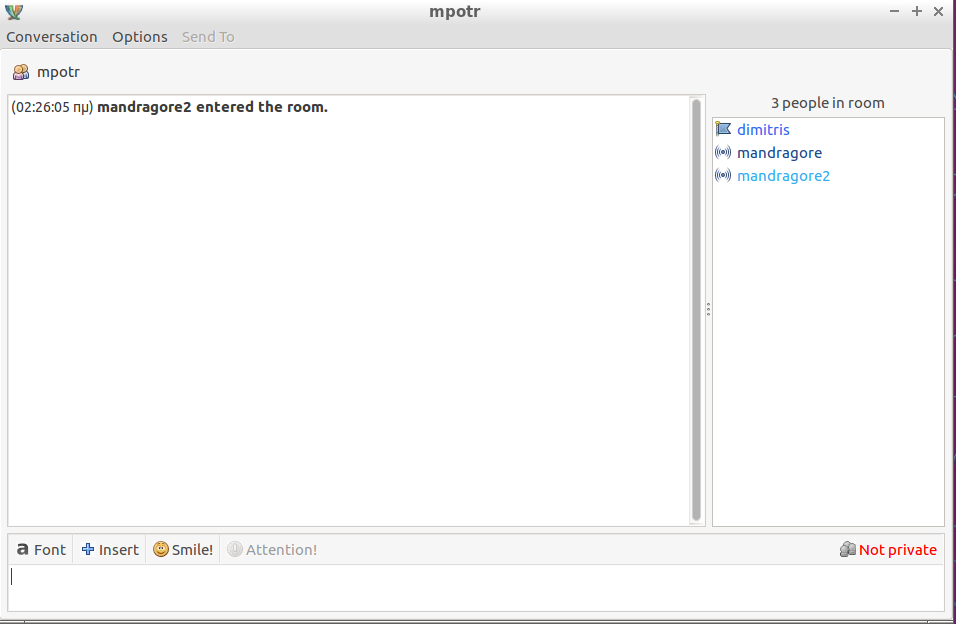
\includegraphics[scale=0.4]{not_started_unverified.png}

By clicking on the mpOTR button a user has the option to start a private conversation.
If he chooses to do so this is what he sees.

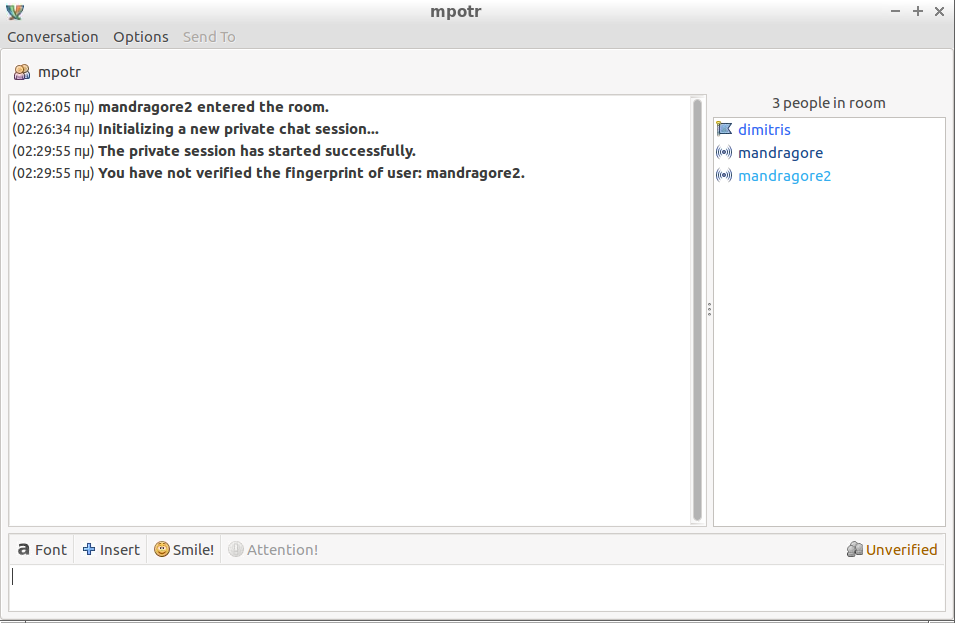
\includegraphics[scale=0.4]{started_unverified.png}

And when some texts are exchanged.

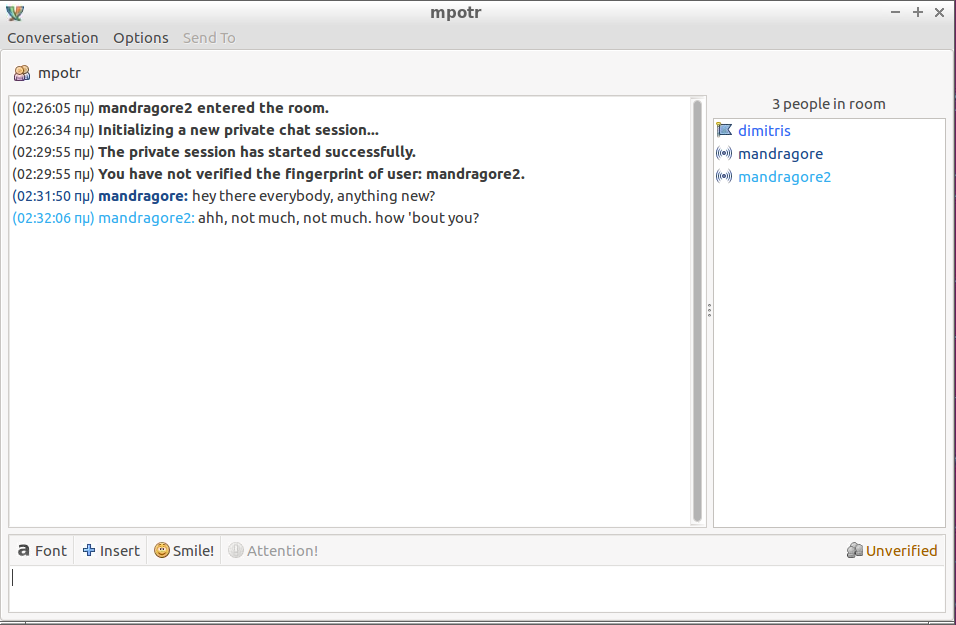
\includegraphics[scale=0.4]{talking_unverified.png}

However, our user (mandragore) hasn't verified another user (mandragore2).
This means that the conversation is unverified.
This is presented to the user in Two ways.
First the mpOTR button has a yellow colour and states that the conversation is "Unverified".
And then, the message "You have not verified user: mandragore2".
This message will be displayed for every unverified user.

In order to verify the user mandragore2, our user clicks on the mpOTR button.
Notice how the "Start private conversation" option is now disabled.

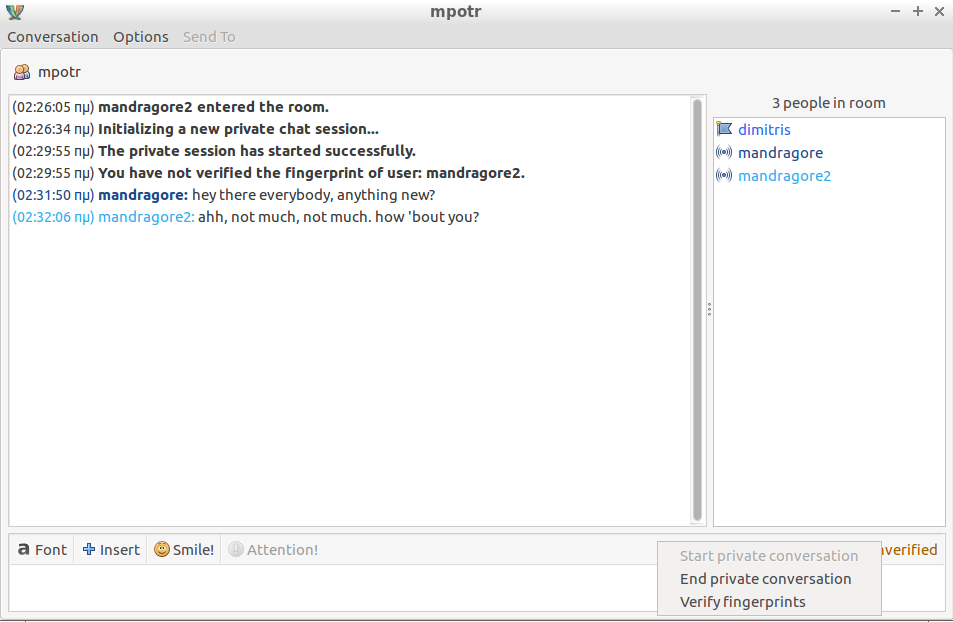
\includegraphics[scale=0.4]{click_mpotr_button_unverified.png}

If he clicks the "Verify fingerprints" option this window opens.

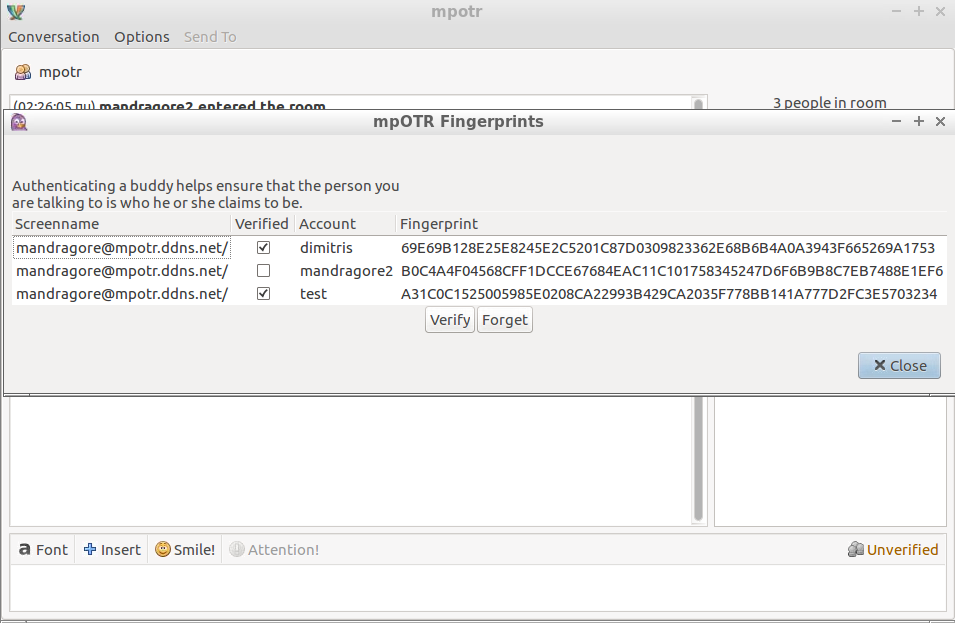
\includegraphics[scale=0.4]{verification_ui_opened_unverified.png}

In this window the user can click on the user he wants to verify and (after he checks the fingerprint) click on the "Verify" button.
The selected user will now be verified.

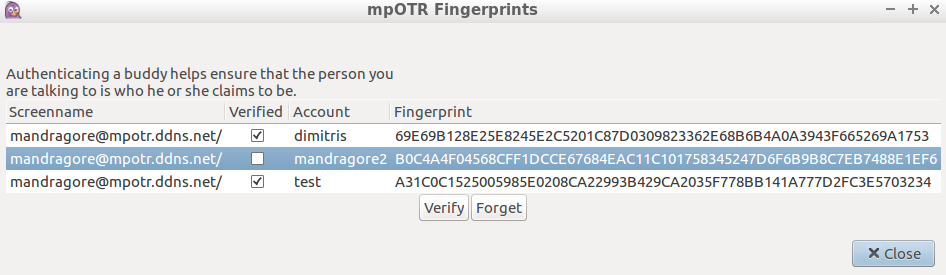
\includegraphics[scale=0.4]{verification_ui_selected_user_unverified.png}

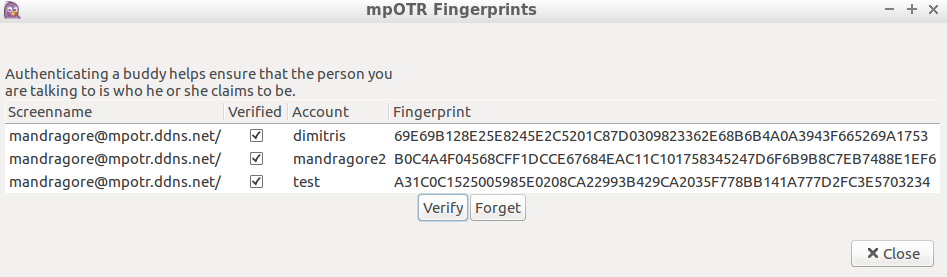
\includegraphics[scale=0.4]{user_verified_unverified.png}

To end the conversation the user clicks on the mpOTR button again and selects the "End private conversation" option.

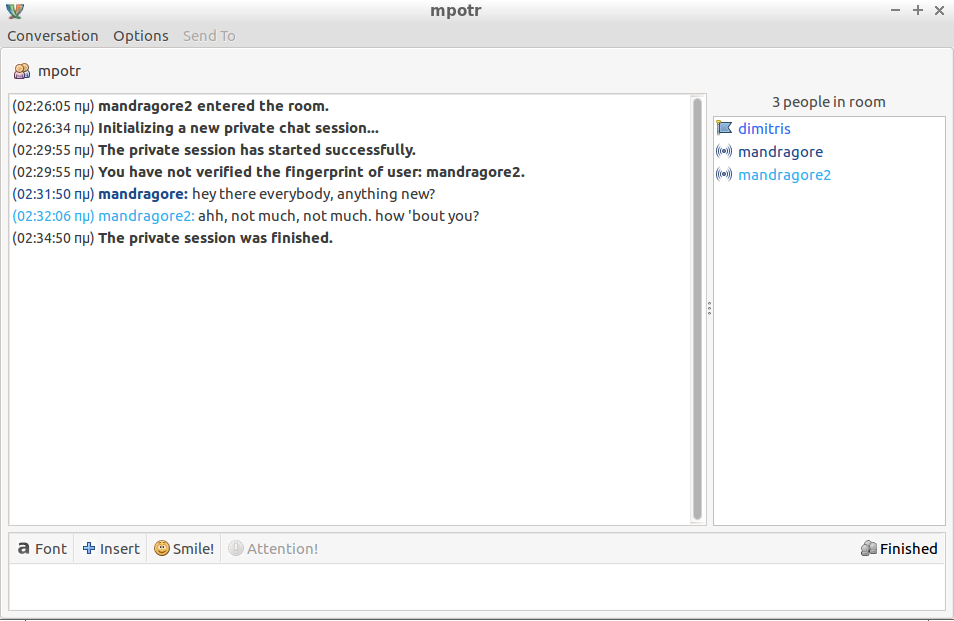
\includegraphics[scale=0.4]{finished_unverified.png}

Now if the user starts another private conversation the new session will be characterised as "Private".

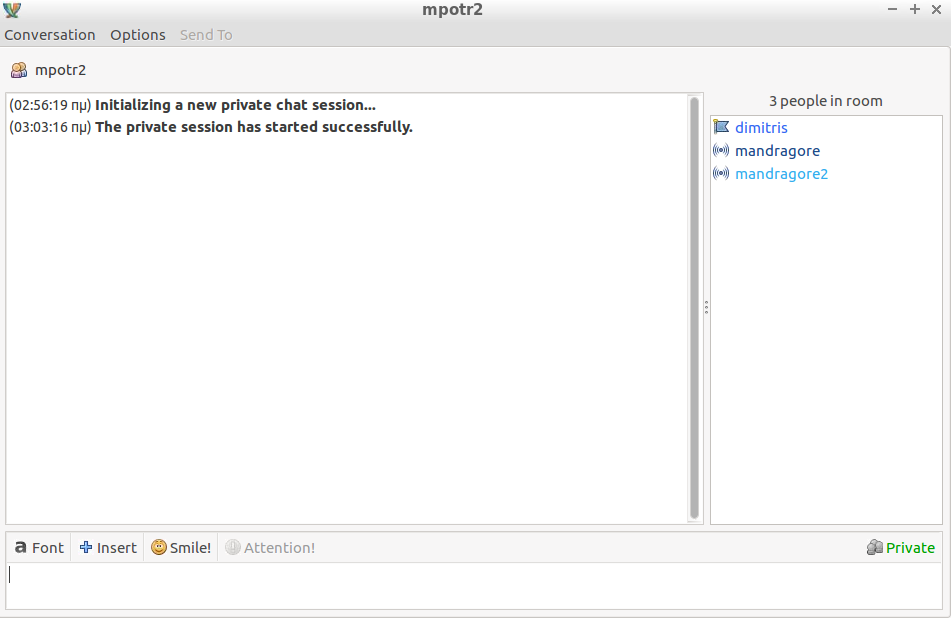
\includegraphics[scale=0.4]{started_verified.png}
%------------------------------------------------

%----------------------------------------------------------------------------------------
%	REFERENCE LIST
%----------------------------------------------------------------------------------------
\bibliographystyle{plain}
\bibliography{ccc_mpotr_pinch}
%----------------------------------------------------------------------------------------

\end{document}
